\documentclass[conference]{IEEEtran}
\IEEEoverridecommandlockouts
% The preceding line is only needed to identify funding in the first footnote. If that is unneeded, please comment it out.
\usepackage{cite}
\usepackage{amsmath,amssymb,amsfonts}
\usepackage{graphicx}
\usepackage{subfigure}
\usepackage{textcomp}
\usepackage{xcolor}

\usepackage{algorithm}
\usepackage{algpseudocode}
\usepackage{array}
\usepackage{bm} % for the bold font Greek symbols in math mode
%\usepackage{breakurl}
\usepackage{color}
\usepackage{comment}
\usepackage{epsfig}
\usepackage{gensymb}
\usepackage{hyperref}
\usepackage{mdwmath} % part of Mark Wooding's powerful
\usepackage{mdwtab}  % tools for math, tables, ...
\usepackage{multirow}
\usepackage{psfrag}
%\usepackage{times}
\usepackage{verbatim}
\usepackage{xspace}
\usepackage{url}
\usepackage{listings}
\usepackage{adjustbox}
\def\BibTeX{{\rm B\kern-.05em{\sc i\kern-.025em b}\kern-.08em
    T\kern-.1667em\lower.7ex\hbox{E}\kern-.125emX}}
\begin{document}

\title{Rate-Distortion Modeling of Synthesizer Immersive Video for 6DoF Interaction}

\author{\IEEEauthorblockN{Yuan Jun Sun}
\IEEEauthorblockA{\textit{dept. name of organization (of Aff.)} \\
\textit{name of organization (of Aff.)}\\
City, Country \\
email address or ORCID}
% \and
% \IEEEauthorblockN{2\textsuperscript{nd} Given Name Surname}
% \IEEEauthorblockA{\textit{dept. name of organization (of Aff.)} \\
% \textit{name of organization (of Aff.)}\\
% City, Country \\
% email address or ORCID}
}

\maketitle

\begin{abstract}
This document is a model and instructions for \LaTeX.
This and the IEEEtran.cls file define the components of your paper [title, text, heads, etc.]. *CRITICAL: Do Not Use Symbols, Special Characters, Footnotes, 
or Math in Paper Title or Abstract.
\end{abstract}

\begin{IEEEkeywords}
component, formatting, style, styling, insert
\end{IEEEkeywords}

\section{Introduction} \label{sec:intro}


Recently, Virtual Reality (VR) becomes increasingly more popular.
It enables a wide array of novel applications in many domains, such as video streaming, computer games, occupational training, healthcare, manufacturing, etc.
The market research also reports that foresee explosive growth of the VR market in the upcoming years~\cite{XR_market}.
More and more companies devote their effort to the VR industry such as Meta~\cite{meta} or Google~\cite{google_AR_VR, MJRD+20}.

\begin{figure}[tbh]
    \centering
    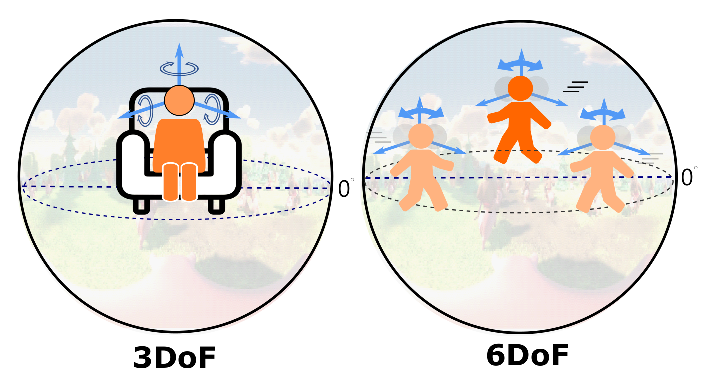
\includegraphics[width=0.46\textwidth]{figs/vr_phase.eps}
    \caption{Difference between 3DoF and 6DoF interactions.}
    \label{fig:vr_phase}
\end{figure}

One way to classify the VR applications is through the different {\em interaction techniques}, including {\em 3DoF} and {\em 6DoF} interactions.
Because of the high popularity of 360{\degree} video streaming services, most users are familiar with the {\em 3DoF} (Degree-of-Freedom) interactions, in which a user's viewport is determined by his/her head/HMD {\em orientation}.
In the 3DoF VR application, the user's position in his/her coordinate such as standing up and walking around, his/her HMD viewport would not reflect the changes of positions.
Therefore, the user will {\em not} feel he/she is moving in the virtual world, leading to an inferior {\em immersive} user experience.
In {\em 6DoF} interactions, the application will render the viewports depending on the user position and orientation. 
Different from the 3DoF interaction, the 6DoF interaction allows users to walk around the virtual world which optimizes the immersive user experience.
Fig.~\ref{fig:vr_phase} illustrates the difference between 3DoF and 6DoF interactions.

Supporting 6DoF Extended Reality (XR) using 360{\degree} videos is not an easy task, because, for every single position, a new 360{\degree} video needs to be captured.
Even if we deploy dense 360{\degree} cameras, users may still miss smooth transitions at the positions between any two adjacent cameras.
Hence, more descriptive 3D representations are required for enabling the truly immersive experience of 6DoF VR applications.
Recently, MPEG-I (Moving Picture Expert Group - Immersive Group) has been actively developing MPEG Immersive Video (MIV) standard~\cite{BDDF+21, MPEG_MIV_web} which can use for 6DoF video compression.
It uses multi-view RGB-D video as the data representation and includes the integrated pipeline for encoding, decoding, synthesizing, and rendering.
The Test Model for Immersive Video (TMIV)~\cite{tmiv_doc,tmiv_gitlab}, which is the reference software of MIV standard, has been released to show a reference implementation of MIV.

Besides, reducing bandwidth and maintaining high view quality is a bottleneck of 6DoF real-time streaming.
Because of the limitation of bandwidth, performing the best quality by adaptive quality model for 6DoF immersive video is quite a challenging work.
There are many existing rate control algorithms for video compression~\cite{PZAB16}\cite{WYTC12}\cite{ZM01}.
Based on the existed rate control algorithms, it is possible to optimize those models to predict the 6DoF video performance.
Although, there are still many effects that could impact the 6DoF video quality, e.g., tile sizes~\cite{JLRL+20}, camera placements, complexity of scenes~\cite{SCB21}, number of groups, synthesizer, and a quantization parameter.
In this paper, we conduct a rate-distortion model (RD-model) to predict the performance of 6DoF immersive video in common situations as we show in Fig.~\ref{fig:RD_model_concept}.
The model will design in an empirical way and aim at some vital TMIV parameters.
The main goal of this model is to generate relevance between TMIV parameters and quality metrics, e.g., PSRN, SSIM, and VMAF.
Once the model generates, it is possible to use on estimate the 6DoF immersive video performance in different camera placements and also use it on real-time 6DoF streaming.

\begin{figure}[tbh]
    \centering
    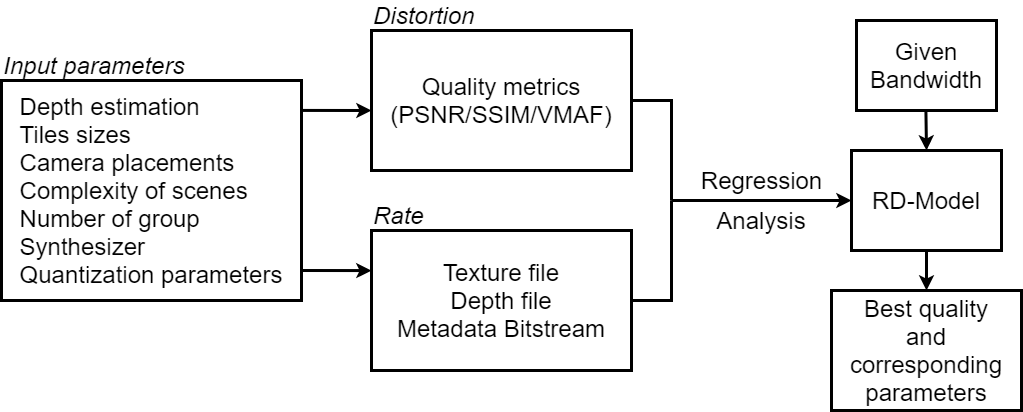
\includegraphics[width=0.46\textwidth]{figs/RD_model_concept}
    \caption{RD-model workflow}
    \label{fig:RD_model_concept}
\end{figure}

% The rest of this paper is organized as follows. We survey the related work in Sec.~\ref{sec:related}, and giving an introduction for MIV standard in Sec.~\ref{sec:TMIV}. Sec.~\ref{sec:implementation} introduce our implementation for experiments. The setup and results of our experiments are shown in Sec.~\ref{sec:experiment}. Finally, we conclude this paper and list some future work in Sec.~\ref{sec:conclusion}

\section{Related Work} \label{sec:related}

{\bf Objective quality assessment} of live immersive video streaming has been
conducted to understand how different settings affect the target view quality.
For example, Cai et al.~\cite{CWQP+21} compared the performance resulted by
using different 2D video codecs to encode depth video in 6DoF streaming. 
Sebastian et al.~\cite{SH17} conducted a similar
study on depth video compression.  In contrast, Szekielda et al.~\cite{SDM21}
studied the implications of 2D encoding parameters on both RGB and depth
videos. Software components other than 2D video codecs have also been
exercised. For example, Fachada et al.~\cite{FBSL18} focused on the impact of
different synthesizers under linear versus planar camera placement.  Pre- or
post-processing of the RGB and depth videos for higher coding efficiency was
also investigated. For example, Jeong et al.~\cite{JLRL+20} proposed to
downsample the RGB video and upsample the depth video to increase the coding
efficiency.  Salahieh et al.~\cite{SBB19} compared the performance of MIV
reference software, called Test Model of Immersive Video (TMIV)~\cite{tmiv_doc}
in the 3D domain. In particular, they considered different settings, including
{\em single-} versus {\em multi-pass synthesis} and {\em MIV} versus {\em MIV
View modes}. 
Last, the impacts of
different camera (source view) densities on synthesized target view quality
were evaluated in Ray et al.~\cite{RJL18}. They concluded that higher camera
densities lead to better perceived quality. Compared to our work, the
aforementioned studies have two major limitation. First, almost all of them (except Ray et al.~\cite{RJL18})
employed existing scene/trajectory datasets. 
Second, none of them considered  {\em continuous} 6DoF trajectories of
source {\em and} target views. The closest setup to continuous 6DoF
trajectories was the {\em discrete} camera locations/orientations adopted in Fachada
et al.~\cite{FBSL18} and Ray et al.~\cite{RJL18}. {\em Our AirSim-based data
collection tools offer the opportunity to generate large and flexible datasets
with real 6DoF source/target trajectories.}

\subsection{Synthesized video}
Basel Salahieh \cite{SCB21} evaluate the performance of the object-based solution. Their results show the pixel rate saving and bitrate distortion in the object-based situation.
Xavier Corbillon \cite{CDSF18} implemented a 6DoF VR application with a multi-camera system and analyzed two extreme optimal algorithms. Their results show that tiling is able to improve the service performance and the high cost for the proactive optimizing strategies
By the previous experiments, both 6DoF video quality and bitrate have a negative correlation with QP.
\section{MPEG Immersive Video Standard}\label{sec:TMIV}

In this section, we briefly introduce the workflow and components of MIV codec~\cite{tmiv_doc,BDDF+21}.

\begin{figure}[tbh]
    \centering
    \subfigure[]{
        \label{fig:TMIV_encode}
        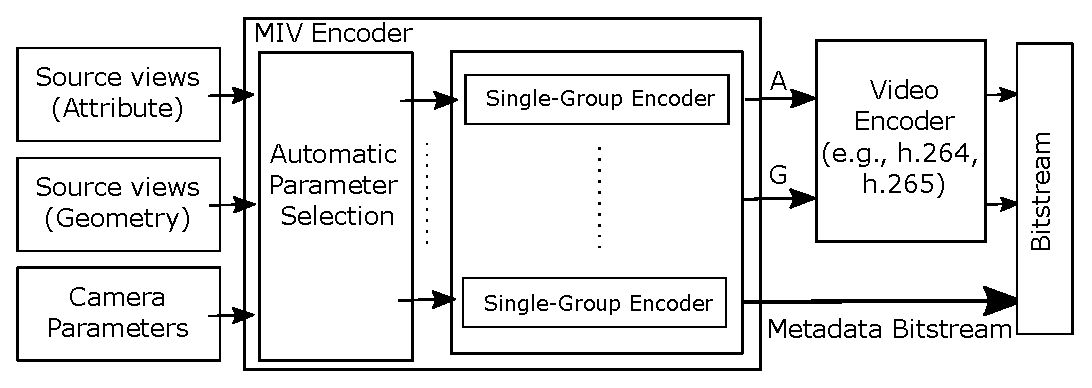
\includegraphics[width=.48\textwidth]{figs/TMIV_encode.eps}
    }
    \\
    \subfigure[]{
        \label{fig:TMIV_decode}
        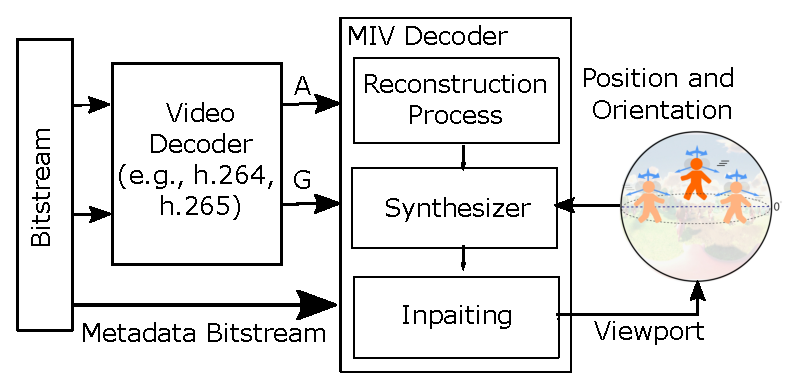
\includegraphics[width=.42\textwidth]{figs/TMIV_decode.eps}
    }
    \caption{The high-level overview of process flow of TMIV: (a) Encoder and (b) Decoder.}
    \label{fig:TMIV_codec}
\end{figure}

Fig.~\ref{fig:TMIV_encode} shows the high-level workflow of MIV encoder. The inputs of MIV encoder are {\em source views}. Each source view is composed of attribute (texture) videos, geometric (depth) videos, and camera parameters. MIV encoder do the following process to compress source views:
\begin{itemize}
    \item {\bf Automatic parameter selection.} MIV encoder automatically calculate the parameters for compression, e.g., assessing geometric video quality, splitting source views into multiple group according to configuration, and labeling source views in each group.
    \item {\bf Single-group encoders.} MIV encoder encodes each group of source views separately. In each group, 
    the encoder chooses several views as the basic view according to the label of source view, and remove the duplicate area in other source views. The basic view and remaining area of other views are packed into rectangle video frames, which are called {\em atlases}. Fig.~\ref{fig:atlas_example} show the example of atlases. 
\end{itemize}

\begin{figure}
    \centering
    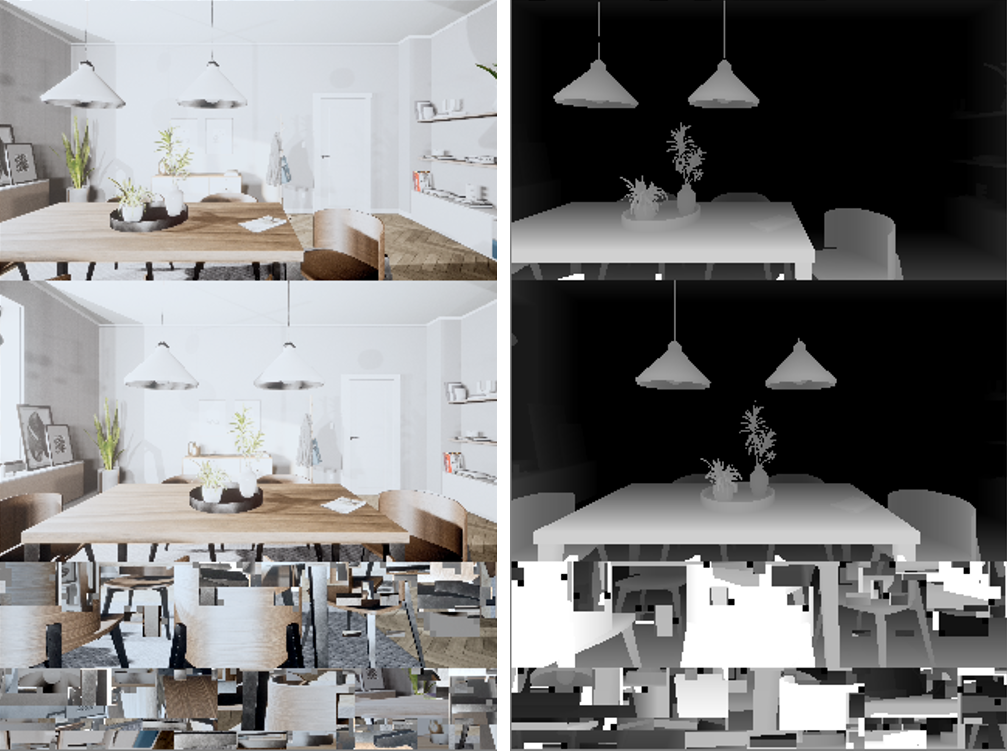
\includegraphics[width=.38\textwidth]{figs/atlas_example.png}
    \caption{The example of atlases. The left picture is attribute atlas, and the right picture is geometric altas.}
    \label{fig:atlas_example}
\end{figure}

The outputs of MIV encoder are attribute atlases, geometric atlases, and metadata bitstream. The atlases are further compressed by video codec, and multiplexed with metadata bitstream as a single bitstream.

Fig.~\ref{fig:TMIV_decode} shows the high-level workflow of MIV decoder. The inputs pf MIV decoder is the bitstream contains atlases bitstream, and metadata bitstream. The video decoder first be employed to decompress attribute atlases and geometric atlases. After that MIV decoder do the following process to decompress altases and synthesize the user's viewport.
\begin{itemize}
    \item {\bf Reconstruction process.} The MIV decoder reconstruct the source view by using the data in atlases.
    \item {\bf Synthesizer.} The MIV decoder employ view synthesis techniques to synthesize the user's viewport according to user's position and orientation. Specifically, the synthesizer warp the pixel of each source view to user's viewport according to depth information, and blending the pixel values from each source views.
    \item {\bf Inpainting.}  After synthesis, the synthesized result may contain holes without information. The inpainting process uses the information from neighbor pixels to calculate pixel value for holes.
\end{itemize}
The outputs of MIV decoder are user's viewport synthesized according to user's position and orientation.

\section{Conclusion} \label{sec:conclusion}




\bibliographystyle{IEEEtran}
\bibliography{./refs}


\end{document}
